\chapter{Image Processing}  \label{chapt:ip}
This chapter deals with the filter developed for the image. First the design flow of Vivado HLS is shown and then how an IP core is generated from a C/C++ code. Then the sobel algorithm is explained and how it was programmed. Finally, the scalability of the filter is discussed. 

\section{Design Flow}
In Vivado HLS it is possible to translate the C/C++ code into VHDL and generate an IP core for Vivado HLx. To ensure that the algorithm is correct, it can be validated in various steps. These steps are the design flow of Vivado HLS and are shown in figure \ref{fig:hls_design_flow}.
First of all, the C/C++ algorithm can be tested in a simulation. This requires a testbench in addition to the C/C++ algorithm. As soon as the algorithm works satisfyingly the design can be run through synthesis and generating a RTL design in VHDL. VHDL design can be verified in an RTL simulation. The RTL simulation must match the C/C++ simulation. If this is the case, an IP core can be generated from the VHDL code and used in the Vivado HLx \cite{vivado_hls}.
%IP Integrator erklären, Block Design, ...

\begin{figure}[tb!]
    \centering
    % \tikzsetnextfilename{system-overview}
\begin{tikzpicture}[
    rounded corners=0mm,
]
    %coordinates
    \coordinate (orig)      at (0,0);
    \coordinate (test)      at (-3,0);
    \coordinate (alg)       at (3,0);
    \coordinate (c_sim)     at (0,-1);
    \coordinate (c_synth)   at (0,-2);
    \coordinate (VHDL)      at (0,-3);
    \coordinate (rtl_sim)   at (0,-4);
    \coordinate (ip)        at (0,-5);
    \coordinate (hlx)       at (0,-6);

    %nodes
    \node[draw, fill=white, minimum width=4cm, minimum height=0.6cm, anchor=south, text width=3.8cm, align=center, rounded corners=3mm] (A) at (test) {C/C++ Testbench};
    \node[draw, fill=white, minimum width=4cm, minimum height=0.6cm, anchor=south, text width=3.8cm, align=center, rounded corners=3mm] (B) at (alg) {C/C++ Algorithm};
    \node[draw, fill=white, minimum width=4cm, minimum height=0.6cm, anchor=south, text width=3.8cm, align=center] (C) at (c_sim) {C/C++ Simulation};
    \node[draw, fill=white, minimum width=4cm, minimum height=0.6cm, anchor=south, text width=3.8cm, align=center] (D) at (c_synth) {C/C++ Synthesis};
    \node[draw, fill=white, minimum width=4cm, minimum height=0.6cm, anchor=south, text width=3.8cm, align=center, rounded corners=3mm] (E) at (VHDL) {VHDL};
    \node[draw, fill=white, minimum width=4cm, minimum height=0.6cm, anchor=south, text width=3.8cm, align=center] (F) at (rtl_sim) {RTL Simulation};
    \node[draw, fill=white, minimum width=4cm, minimum height=0.6cm, anchor=south, text width=3.8cm, align=center] (G) at (ip) {Package IP};
    \node[draw, fill=white, minimum width=4cm, minimum height=0.6cm, anchor=south, text width=3.8cm, align=center] (H) at (hlx) {Vivado HLx};

    %path
    \path [draw,-] (A) -- (B);
    \path[draw,-{Latex[length=2.5mm]}] (A) -| (C);
    \path[draw,-{Latex[length=2.5mm]}] (C.east) -- ++(3.5,0) |- (B.east);
    \path[draw,-{Latex[length=2.5mm]}] (C) -- (D);
    \path[draw,-{Latex[length=2.5mm]}] (D) -- (E);
    \path[draw,-{Latex[length=2.5mm]}] (E) -- (F);
    \path[draw,-{Latex[length=2.5mm]}] (E.west) -- ++(-0.5,0) |- (G.west);
    \path[draw,-{Latex[length=2.5mm]}] (F.east) -- ++(3.5,0) |- (B.east);
    \path[draw,-{Latex[length=2.5mm]}] (G) -- (H);


\end{tikzpicture}
    \caption{Vivado HLS design flow}
    \label{fig:hls_design_flow}
\end{figure}


\section{Requirements}
%Was ist für die Sobel-Edge-Detection notwendig und wie muessen die Pixelwerte vorliegen

The Sobel filter has some requirements. A grayscale image is required for edge detection. As already described in chapter \ref{chapt:mission_imageprocessing} the Sobel filter depends on its neighbor pixels. Therefore, the entire image does not have to be present. These are the most important requirements of this filter.


\section{Concept} \label{chapt:concept}
%Das Konzept des Programmierten Filters. Wie das Filter genau funktioniert. 

\begin{figure}[b]
    \centering
    \begin{adjustbox}{width=0.5\textwidth}
    	% \tikzsetnextfilename{system-overview}
\begin{tikzpicture}[
    rounded corners=0mm,
]
    %coordinates
    \coordinate (orig)      at (0,0);
    \coordinate (gray)      at (0,0);
    \coordinate (sob_x)     at (-2,-1);
    \coordinate (sob_y)     at (2,-1);
    \coordinate (grad)      at (0,-2);
    \coordinate (hyst)      at (0,-3);
    \coordinate (o_img)     at (0,-4);

    %nodes
    \node[draw, fill=white, minimum width=3cm, minimum height=0.6cm, anchor=south, text width=2.8cm, align=center] (A) at (gray) {Grayscale Image};
    \node[draw, fill=white, minimum width=3cm, minimum height=0.6cm, anchor=south, text width=2.8cm, align=center] (B) at (sob_x) {Sobel X};
    \node[draw, fill=white, minimum width=3cm, minimum height=0.6cm, anchor=south, text width=2.8cm, align=center] (C) at (sob_y) {Sobel Y};
    \node[draw, fill=white, minimum width=3cm, minimum height=0.6cm, anchor=south, text width=2.8cm, align=center] (D) at (grad) {Gradient};
    \node[draw, fill=white, minimum width=3cm, minimum height=0.6cm, anchor=south, text width=2.8cm, align=center] (E) at (hyst) {Hysteresis};
    \node[draw, fill=white, minimum width=3cm, minimum height=0.6cm, anchor=south, text width=2.8cm, align=center] (F) at (o_img) {Output Image};

    %path
    \path[draw,-{Latex[length=2.5mm]}] (A) -- (B);
    \path[draw,-{Latex[length=2.5mm]}] (A) -- (C);
    \path[draw,-{Latex[length=2.5mm]}] (B) -- (D);
    \path[draw,-{Latex[length=2.5mm]}] (C) -- (D);
    \path[draw,-{Latex[length=2.5mm]}] (D) -- (E);
    \path[draw,-{Latex[length=2.5mm]}] (E) -- (F);

    \node at (-1.5,-1.2) {\tiny Gx};
    \node at (1.5,-1.2) {\tiny Gy};

\end{tikzpicture}
    \end{adjustbox}
    \caption{Concept of the Sobel edge detection algorithm}
    \label{fig:sobel}
\end{figure}
	
The algorithm uses a convolution applying a 3x3 matrix, which generates a gradient image from the grayscale image. This is used to display high frequencies in the image with gray values. The areas of greatest intensity are where the brightness of the input image changes most rapidly and thus represents the largest edges. The concept of the Sobel algorithm is shown in figure \ref{fig:sobel}. 

Only a 3x3 section of the grayscale image $I$ is used for each pixel. With a 3x3 matrix, merely the nine neighboring pixels are used. The filter matrix are the approximations of the weighted derivatives in horizontal and vertical direction. \\

\noindent\begin{minipage}{.5\linewidth}

\textbf{Horizontal changes:}
\begin{equation}
    G_{x} = I * \begin{bmatrix}
                -1 & 0 & 1 \\ 
                -2 & 0 & 2 \\ 
                -1 & 0 & 1
                \end{bmatrix}
    \label{eq:gx_derivative}
\end{equation} \\

\end{minipage}%
\begin{minipage}{.5\linewidth}

\textbf{Vertical changes:}
\begin{equation}
    G_{y} = I * \begin{bmatrix}
                -1 & -2 & -1 \\ 
                0 & 0 & 0 \\ 
                1 & 2 & 1
                \end{bmatrix}
    \label{eq:gx_derivative}
\end{equation} \\

\end{minipage}


The gradient is calculated for each pixel of the image. The theory says that the root of squares of the two derivatives should be used:
\begin{equation}
    G = \sqrt{ G_{x}^{2} + G_{y}^{2}}
    \label{eq:g_square_root}
\end{equation}
\\

In order to save resources on the FPGA, the gradient can also be calculated with the absolute values of the derivatives:
\begin{equation}
    G = \left |G_{x}  \right | + \left |G_{y}  \right |
    \label{eq:g_abs}
\end{equation}
\\

The final stage of the Sobel edge detector is referred to as hysteresis. If the result $G$ is greater/lower than the maximum/minimum value, the result is set to this threshold value \cite{sobel_matrix}.


\section{Implementation}
The implementation of the Sobel edge detection is shown below. The code has the same sequence as shown in figure \ref{fig:sobel}. The edge detection is implemented as a function. For the function only the required pixels have to be passed. The two filter matrixes are defined in the header file. The return value is the gradient, in this case the variable \texttt{sum}. \\


Listing \ref{lst:matrix} contains the mirrored filter matrix for calculating horizontal changes. The matrix was mirrored because it is a convolution with the image.

\begin{minipage}{\textwidth}
\begin{lstlisting}[style=CStyle, caption=Filter matrix defined in header, label=lst:matrix]
// Filter-Matrix
static int sobel_x [3][3] = {{1,0,-1},
					  	  	 					 {2,0,-2},
												 		 {1,0,-1}};
\end{lstlisting}
\end{minipage}
\\

As can be seen in the filter matrix, the middle column has the weighting zero. Therefore, these pixels do not have to be included in the calculation and only six pixels have an impact on the calculation.

\begin{minipage}{\textwidth}
\begin{lstlisting}[style=CStyle , caption=Calculation of derivative, label=lst:derivative]
gx = 	sobel_x[0][0] * pixel_00 +
			sobel_x[1][0] * pixel_10 +
			sobel_x[2][0] * pixel_20 +
			sobel_x[0][2] * pixel_02 +
			sobel_x[1][2] * pixel_12 +
			sobel_x[2][2] * pixel_22;
\end{lstlisting}
\end{minipage}
\\

In this code section, the absolute value of each derivative is calculated and the gradient is generated.

\begin{minipage}{\textwidth}
\begin{lstlisting}[style=CStyle , caption=Evaluate the absolute value and the gradient, label=lst:gradient]
gx = gx < 0 ? -gx : gx; // abs(gx)
gy = gy < 0 ? -gy : gy; // abs(gy)
sum = gx + gy;
\end{lstlisting}
\end{minipage}
\\

Finally, the hysteresis is adjusted with an upper and lower threshold value. The calculated gradient can be returned as a new pixel.

\begin{minipage}{\textwidth}
\begin{lstlisting}[style=CStyle , caption=Threshold, label=lst:threshold]
sum = sum > 255 ? 255:sum; // max threshold
sum = sum < 0 ? 0 : sum; 	 // min threshold
\end{lstlisting}
\end{minipage}

\clearpage
\section{Scalability}
%Was wurde gemacht, damit der Filter im FPGA auf mehrere aufgeteilt werden kann.
In order to take advantage of the area on the FPGA and increase the throughput, the image can be split into blocks. A Sobel algorithm can be loaded with an image block to calculate it. Figure \ref{fig:impl_sobel} shows a model to calculate one row of pixels. On the left side is the input memory. A row of pixels is loaded into each one. Three pixels from every input memory are loaded into the Sobel filter. With these nine pixels a new pixel can be calculated and stored in the output memory.
This splitting into blocks guarantees a very simple scalability of the image within an FPGA and also on multiple FPGAs. The pixel data for a filter and the calculated pixel data must only be handled correctly. Figure \ref{fig:impl_sobel2} shows how this scalability can be used to implement multiple filters. 

\begin{figure}[h!]
    \centering
    \begin{adjustbox}{width=0.8\textwidth}
        % \tikzsetnextfilename{system-overview}
\begin{tikzpicture}[
    rounded corners=0mm,
]
    %coordinates
    \coordinate (orig)      at (0,0);
    \coordinate (sob)      at (0,-0.7);
    \coordinate (mem1)     at (-3.5,1);
    \coordinate (mem2)     at (-3.5,0);
    \coordinate (mem3)      at (-3.5,-1);
    \coordinate (mem4)      at (3.5,0);

    %nodes
    \node[draw, fill=white, minimum width=2cm, minimum height=2cm, anchor=south, text width=1.8cm, align=center] (A) at (sob) {Sobel Filter};
    \node[draw, fill=white, minimum width=3cm, minimum height=0.6cm, anchor=south, text width=2.8cm, align=center] (B) at (mem1) {Memory (row 0)};
    \node[draw, fill=white, minimum width=3cm, minimum height=0.6cm, anchor=south, text width=2.8cm, align=center] (C) at (mem2) {Memory (row 1)};
    \node[draw, fill=white, minimum width=3cm, minimum height=0.6cm, anchor=south, text width=2.8cm, align=center] (D) at (mem3) {Memory (row 2)};
    \node[draw, fill=white, minimum width=3cm, minimum height=0.6cm, anchor=south, text width=2.8cm, align=center] (E) at (mem4) {Memory (row 0)};

    %path
    \path[draw,-{Latex[length=2.5mm]}] (B.east) -- ++(0.5,0) |- ($(A.180) + (0,0.5)$);
    \path[draw,-{Latex[length=2.5mm]}] (C) -- (A);
    \path[draw,-{Latex[length=2.5mm]}] (D.east) -- ++(0.5,0) |- ($(A.180) + (0,-0.5)$);
    \path[draw,-{Latex[length=2.5mm]}] (A) -- (E);

\end{tikzpicture}
    \end{adjustbox}
    \caption{Implementation of the Sobel filter in the FPGA}
    \label{fig:impl_sobel}
\end{figure}

\begin{figure}[h!]
    \centering
    \begin{adjustbox}{width=0.8\textwidth}
    	% \tikzsetnextfilename{system-overview}
\begin{tikzpicture}[
    rounded corners=0mm,
]
    %coordinates
    \coordinate (orig)      at (0,0);
    \coordinate (sob)      at (0,-0.7);
    \coordinate (mem1)     at (-3.5,1);
    \coordinate (mem2)     at (-3.5,0);
    \coordinate (mem3)      at (-3.5,-1);
    \coordinate (mem4)      at (3.5,0);

    \coordinate (sob2)      at (0,-3.2);
    \coordinate (mem21)      at (-3.5,-3);
    \coordinate (mem22)      at (3.5,-2.5);

    \coordinate (sob3)      at (0,-5.7);
    \coordinate (mem31)      at (-3.5,-5.5);
    \coordinate (mem32)      at (3.5,-5);



    %nodes
    \node[draw, fill=white, minimum width=2cm, minimum height=2cm, anchor=south, text width=1.8cm, align=center] (A) at (sob) {Sobel Filter};
    \node[draw, fill=white, minimum width=3cm, minimum height=0.6cm, anchor=south, text width=2.8cm, align=center] (B) at (mem1) {Memory (row 0)};
    \node[draw, fill=white, minimum width=3cm, minimum height=0.6cm, anchor=south, text width=2.8cm, align=center] (C) at (mem2) {Memory (row 1)};
    \node[draw, fill=white, minimum width=3cm, minimum height=0.6cm, anchor=south, text width=2.8cm, align=center] (D) at (mem3) {Memory (row 2)};
    \node[draw, fill=white, minimum width=3cm, minimum height=0.6cm, anchor=south, text width=2.8cm, align=center] (E) at (mem4) {Memory (row 0)};

    \node[draw, fill=white, minimum width=2cm, minimum height=2cm, anchor=south, text width=1.8cm, align=center] (F) at (sob2) {Sobel Filter};
    \node[draw, fill=white, minimum width=3cm, minimum height=0.6cm, anchor=south, text width=2.8cm, align=center] (G) at (mem21) {Memory (row 3)};
    \node[draw, fill=white, minimum width=3cm, minimum height=0.6cm, anchor=south, text width=2.8cm, align=center] (H) at (mem22) {Memory (row 1)};

    \node[draw, fill=white, minimum width=2cm, minimum height=2cm, anchor=south, text width=1.8cm, align=center] (I) at (sob3) {Sobel Filter};
    \node[draw, fill=white, minimum width=3cm, minimum height=0.6cm, anchor=south, text width=2.8cm, align=center] (J) at (mem31) {Memory (row 4)};
    \node[draw, fill=white, minimum width=3cm, minimum height=0.6cm, anchor=south, text width=2.8cm, align=center] (K) at (mem32) {Memory (row 2)};


    %path
    \path[draw,-{Latex[length=2.5mm]}] (B.east) -- ++(0.5,0) |- ($(A.180) + (0,0.5)$);
    \path[draw,-{Latex[length=2.5mm]}] (C) -- (A);
    \path[draw,-{Latex[length=2.5mm]}] (D.east) -- ++(0.5,0) |- ($(A.180) + (0,-0.5)$);
    \path[draw,-{Latex[length=2.5mm]}] (A) -- (E);

    \path[draw,-{Latex[length=2.5mm]}] (C.east) -- ++(0.4,0) |- ($(F.180) + (0,0.5)$);
    \path[draw,-{Latex[length=2.5mm]}] (D.east) -- ++(0.3,0) |-  ($(F.180) + (0,0)$);
    \path[draw,-{Latex[length=2.5mm]}] (G) -- ($(F.180) + (0,-0.5)$);
    \path[draw,-{Latex[length=2.5mm]}] (F) -- (H);

    \path[draw,-{Latex[length=2.5mm]}] (D.east) -- ++(0.3,0) |- ($(I.180) + (0,0.5)$);
    \path[draw,-{Latex[length=2.5mm]}] (G.east) -- ++(0.2,0) |-  ($(I.180) + (0,0)$);
    \path[draw,-{Latex[length=2.5mm]}] (J) -- ($(I.180) + (0,-0.5)$);
    \path[draw,-{Latex[length=2.5mm]}] (I) -- (K);

    \node at (-1.575,0.3) [circle, fill, inner sep=0.7pt] {};
    \node at (-1.675,-0.7) [circle, fill, inner sep=0.7pt] {};
    \node at (-1.675,-2.2) [circle, fill, inner sep=0.7pt] {};
    \node at (-1.775,-2.7) [circle, fill, inner sep=0.7pt] {};



\end{tikzpicture}
    \end{adjustbox}
    \caption{Scalability of the Sobel filter in the FPGA}
    \label{fig:impl_sobel2}
\end{figure}



\section{Svynthesis}
Before optimizing the C/C++ code, the result must be analyzed. If the C/C++ code is synthesized without optimizations, the throughput will not be better than in a normal C/C++ program. For example, the compiler will process the loops sequentially. By adding attributes, directives, or pragmas the problem can be solved and the code can be adapted to hardware. For C/C++ code, pragmas are used to improve the throughput, latency or resources \cite{vivado_synthesis}. 


\subsection{Pragma}
Loops are often represented in the code to prepare and process the pixels in the proper order. The most important two pragmas for loops are \texttt{pipline} and \texttt{unroll} \cite{pragma}. These two functions improve the hardware's performance by exploiting the parallelism between loop iterations. \\

\textbf{Loop Piplining:} For a normal loop execution, processing is sequential and the next iteration of the loop cannot begin until the previous one is completed. Loop pipelining allows to start the next iteration in advance. 
As can be seen in figure \ref{fig:pipelining}, the loop has a latency of three clock cycles for the whole iteration. However, with the pragma \texttt{\#pragma HLS pipeline} the latency can be reduced to one clock cycle.
The pragma \texttt{pipline} is recursive and unrolls automatically all loops in the hierarchy. 
Loop pipelining is used if the data is not yet fully available. This means, as seen in figure \ref{fig:pipelining}, when for example it is necessary to load the data from a memory at first \cite{pragma}. \\


\begin{figure}[h!]
    \centering
    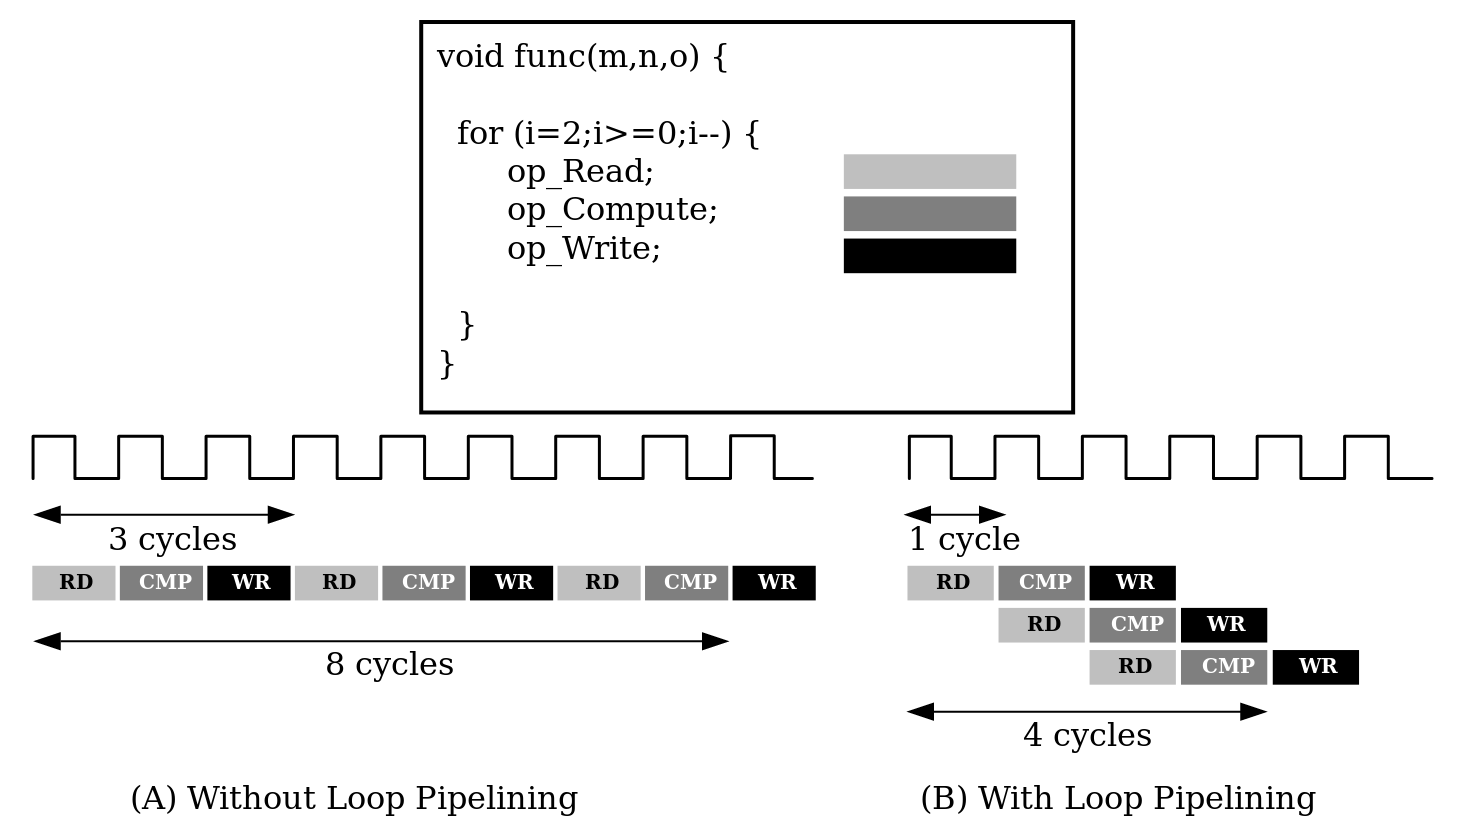
\includegraphics[width=0.8\textwidth]{images/image_processing/pipelining.png}
    \caption{Comparison of loop pipelinging \cite{pragma}}
    \label{fig:pipelining}
\end{figure}

\clearpage
\textbf{Loop Unrolling:} With the pragma \texttt{\#pragma HLS unroll} a loop can be parallelized. This means that the entire loop can be processed in parallel. With a factor, the parallelism can be controlled. By default, the entire loop is parallelized. 
Loop unrolling is used when the data is available and they are not loaded or already loaded for the entire loop \cite{pragma}. 
In this code section, the loop is parallelized with a factor of 2:

\begin{lstlisting}[style=CStyle , caption=Loop unrolling with a factor of 2 \cite{pragma}]
for(int i = 0; i < X; i++) {
  #pragma HLS unroll factor=2
  a[i] = b[i] + c[i];
}
\end{lstlisting}

The model of unrolling can be seen here:
\begin{lstlisting}[style=CStyle , caption=Loop unrolling with a factor of 2 \cite{pragma}]
for(int i = 0; i < X; i += 2) {
  a[i] = b[i] + c[i];
  if (i+1 >= X) break;
  a[i+1] = b[i+1] + c[i+1];
}
\end{lstlisting}


\subsection{Analysis}
Code analysis is important for optimizing code and improving performance. This section shows how to analyze a code. At Vivado HLS there is a report and graphical analysis to identify mistakes. 

\subsubsection*{Report Analysis}
The Sobel filter with and without pragmas is placed in contrast (see table \ref{tab:analysis}). The loop pragmas were optimized for throughput. With each new clock cycle a new iteration is started. As a result, the memory requirements increase as more variables have to be stored. 
The graphical analysis does not make any sense when processing without pragmas. Because of the nesting of multiple loops, the compiler can no longer work properly. In the next example, the graphical analysis makes much more sense .\\

\begin{table}[h!]
    \centering
    \begin{tabular}{ l l l }
    	\toprule
         & {without Pragma} & {with Pragma} \\ 
        \midrule
        Latency & 23'471 - 31'631 & 515 \\
        Throughput & 0.018 Pixel / Clk & 1 Pixel / Clk \\ 
        FF & 2783 & 3451 \\ 
        LUT & 2574 & 2512 \\ 
        \bottomrule
    \end{tabular}
    \caption{Report analysis (iterations: 510)}
    \label{tab:analysis}
\end{table}

\clearpage
\subsubsection*{Graphical Analysis}
Graphical analysis in the Vivado HLS is very useful. The goal was to improve memory access and thereby increasing throughput. In the first programming an error occurred and during the analysis the following figure \ref{tab:wrong_code} appeared. The figure shows that at each iteration it accesses the memory twice. Two clock cycles are required to read out one word from a BRAM. In the first, the address is sent to the BRAM and in the second, the data is read out \cite{bram}. In figure \ref{tab:wrong_code} however, the addressing to the BRAM occures in clock 1 (C1). In Clock 2 (C2) the pixels are read out and the second addressing follows for the pixels which are read out in Clock 3 (C3). However, there should be only one memory access at each iteration. At an iteration size of 510, this resulted in a latency of 1024 clock cycles. \\

By positioning the memory access in front of the loop, these two memory accesses could be avoided with each iteration. The result of the analysis is in figure \ref{tab:correct_code}. The new latency has been reduced to 515 clock cycles but the initialization was bigger, because the memory access is before the loop (C0 and C1).


\begin{table}[h!]
\setlength{\aboverulesep}{0pt}
\setlength{\belowrulesep}{0pt}
\centering
\begin{tabular}{lllll|l|llll}
\hline
\multicolumn{1}{|l|}{C0} & \multicolumn{1}{l|}{C1} & \multicolumn{1}{l|}{C2} & \multicolumn{1}{l|}{C3} & C4 & C5 & \multicolumn{1}{l|}{C6} & \multicolumn{1}{l|}{C7} & \multicolumn{1}{l|}{C8} & \multicolumn{1}{l|}{C9} \\ \hline
\multicolumn{1}{|l|}{\cellcolor[HTML]{9B9B9B}{\color[HTML]{FFFFFF} Init}} & \multicolumn{1}{l|}{\cellcolor[HTML]{9B9B9B}{\color[HTML]{FFFFFF} RD}} & \multicolumn{1}{l|}{\cellcolor[HTML]{9B9B9B}{\color[HTML]{FFFFFF} RD}} & \multicolumn{1}{l|}{\cellcolor[HTML]{9B9B9B}{\color[HTML]{FFFFFF} RD}} & \cellcolor[HTML]{FFFFFF}{\color[HTML]{333333} CALC} & \cellcolor[HTML]{9B9B9B}{\color[HTML]{FFFFFF} WR} & {\color[HTML]{FFFFFF} } & {\color[HTML]{FFFFFF} } &  &  \\ \cmidrule{1-8}
{\color[HTML]{FFFFFF} } & {\color[HTML]{FFFFFF} } & \multicolumn{1}{l|}{{\color[HTML]{FFFFFF} }} & \multicolumn{1}{l|}{\cellcolor[HTML]{9B9B9B}{\color[HTML]{FFFFFF} RD}} & \cellcolor[HTML]{9B9B9B}{\color[HTML]{FFFFFF} RD} & \cellcolor[HTML]{9B9B9B}{\color[HTML]{FFFFFF} RD} & \multicolumn{1}{l|}{\cellcolor[HTML]{FFFFFF}{\color[HTML]{333333} CALC}} & \multicolumn{1}{l|}{\cellcolor[HTML]{9B9B9B}{\color[HTML]{FFFFFF} WR}} &  &  \\ \cmidrule{4-10}
{\color[HTML]{FFFFFF} } & {\color[HTML]{FFFFFF} } & {\color[HTML]{FFFFFF} } &  &  & \cellcolor[HTML]{9B9B9B}{\color[HTML]{FFFFFF} RD} & \multicolumn{1}{l|}{\cellcolor[HTML]{9B9B9B}{\color[HTML]{FFFFFF} RD}} & \multicolumn{1}{l|}{\cellcolor[HTML]{9B9B9B}{\color[HTML]{FFFFFF} RD}} & \multicolumn{1}{l|}{\cellcolor[HTML]{FFFFFF}{\color[HTML]{333333} CALC}} & \multicolumn{1}{l|}{\cellcolor[HTML]{9B9B9B}{\color[HTML]{FFFFFF} WR}} \\ \cmidrule{6-10}
\end{tabular}
\caption{The wrong code with three iterations in the loop}
\label{tab:wrong_code}
\end{table}


\begin{table}[h!]
\setlength{\aboverulesep}{0pt}
\setlength{\belowrulesep}{0pt}
\centering
\begin{tabular}{llll|llll}
\hline
\multicolumn{1}{|l|}{C0} & \multicolumn{1}{l|}{C1} & \multicolumn{1}{l|}{C2} & \multicolumn{1}{l|}{C3} & \multicolumn{1}{l|}{C4} & \multicolumn{1}{l|}{C5} & \multicolumn{1}{l|}{C6} & \multicolumn{1}{l|}{C7} \\ \hline
\multicolumn{1}{|l|}{\cellcolor[HTML]{9B9B9B}{\color[HTML]{FFFFFF} Init}} & \multicolumn{1}{l|}{\cellcolor[HTML]{9B9B9B}{\color[HTML]{FFFFFF} Init}} & \multicolumn{1}{l|}{\cellcolor[HTML]{9B9B9B}{\color[HTML]{FFFFFF} RD}} & \multicolumn{1}{l|}{\cellcolor[HTML]{9B9B9B}{\color[HTML]{FFFFFF} RD}} & \multicolumn{1}{l|}{\cellcolor[HTML]{FFFFFF}{\color[HTML]{333333} CALC}} & \multicolumn{1}{l|}{\cellcolor[HTML]{9B9B9B}{\color[HTML]{FFFFFF} WR}} & {\color[HTML]{FFFFFF} } & {\color[HTML]{FFFFFF} } \\ \cmidrule{1-7}
{\color[HTML]{FFFFFF} } & {\color[HTML]{FFFFFF} } & \multicolumn{1}{l|}{{\color[HTML]{FFFFFF} }} & \multicolumn{1}{l|}{\cellcolor[HTML]{9B9B9B}{\color[HTML]{FFFFFF} RD}} & \multicolumn{1}{l|}{\cellcolor[HTML]{9B9B9B}{\color[HTML]{FFFFFF} RD}} & \multicolumn{1}{l|}{{\color[HTML]{333333} CALC}} & \multicolumn{1}{l|}{\cellcolor[HTML]{9B9B9B}{\color[HTML]{FFFFFF} WR}} & {\color[HTML]{FFFFFF} } \\ \cmidrule{4-8}
{\color[HTML]{FFFFFF} } & {\color[HTML]{FFFFFF} } & {\color[HTML]{FFFFFF} } &  &  \multicolumn{1}{l|}{\cellcolor[HTML]{9B9B9B}{\color[HTML]{FFFFFF} RD}} & \multicolumn{1}{l|}{\cellcolor[HTML]{9B9B9B}{\color[HTML]{FFFFFF} RD}} & \multicolumn{1}{l|}{\cellcolor[HTML]{FFFFFF}{\color[HTML]{333333} CALC}} & \multicolumn{1}{l|}{\cellcolor[HTML]{9B9B9B}{\color[HTML]{FFFFFF} WR}} \\ \cmidrule{5-8}
\end{tabular}
\caption{The correct code with three iterations in the loop}
\label{tab:correct_code}
\end{table}


